\documentclass[utf8]{beamer}

\usepackage[ngerman]{babel}

%\usefonttheme{professionalfonts}
%\usetheme{Madrid}
%\usetheme{AnnArbor}
%\usetheme{CambridgeUS}

\usepackage{amsmath}
\usepackage{amssymb}

\usepackage{microtype}
\usepackage{graphicx}
\usepackage{booktabs}
\usepackage{tabularx}

\usepackage{tikz}

\usepackage[]{algorithm}
\usepackage[]{algorithmic}
\floatname{algorithm}{Algorithmus}

\usepackage[square,sort,comma,numbers]{natbib}

\newcommand{\N}{\mathbb{N}}
\newcommand{\Z}{\mathbb{Z}}
\newcommand{\ggT}{\text{ggT}}

\begin{document}

\title[]{Diskrete Logarithmen}
%\subtitle{Und hier der Untertitel}
\author{Martin Darmüntzel \& Hannes Kleinwort}
\date{\today}
\institute{Universität Rostock}

\begin{frame}
  \titlepage{}
\end{frame}

\begin{frame}[t]{Inhalt}
  \tableofcontents
\end{frame}

\section{Motivation}
\label{sec:motivation}

\begin{frame}{\insertsectionhead}
  \begin{center}
    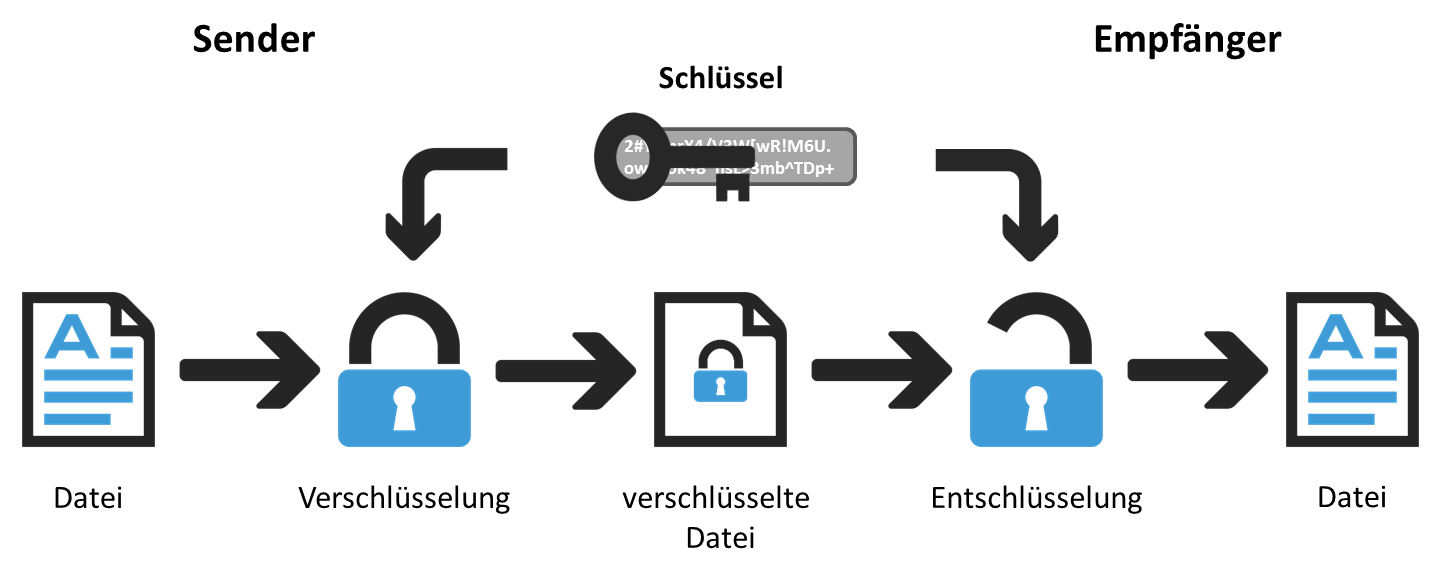
\includegraphics[width=\textwidth]{verschluesselung.png}
  \end{center}
\end{frame}

\section{Mathematische Grundlagen}
\label{sec:mathematische_grundlagen}

\subsection{Kongruenz}
\label{sub:kongruenz}

\begin{frame}{\insertsubsectionhead}
  Zwei ganze Zahlen $a, b$ sind \emph{kongruent} bezüglich eines Moduls $m$,
  wenn sie bei der Division durch $m$ denselben Rest haben. Alternativ kann man
  Kongruenz auch auf den Teilbarkeitsbegriff zurückführen:
  \begin{align*}
    a \equiv b \mod m \Leftrightarrow m \mid (a - b)
  \end{align*}
\end{frame}

\begin{frame}{\insertsubsectionhead}
  \begin{center}
    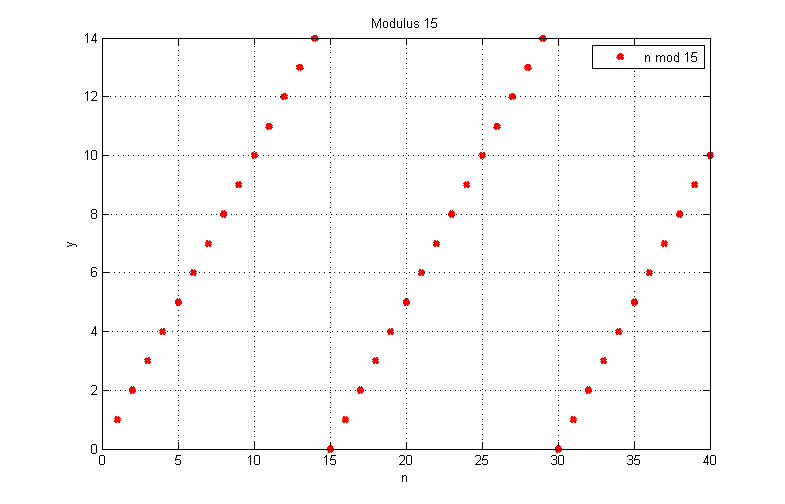
\includegraphics[width=\textwidth]{Modulus.png}
  \end{center}
\end{frame}

\subsection{Gruppe}
\label{sub:gruppe}

\begin{frame}{\insertsubsectionhead}
  Eine Gruppe ist ein Tupel $(G, *)$ mit einer Menge $G$ und einer
  Verknüpfung $*: G \times G \to G$ bzw. $(a, b) \mapsto a * b$, welche
  folgende Axiome erfüllt:
  \begin{enumerate}
    \item Assoziativgesetz: für alle $a,b,c \in G$ gilt: $(a * b) * c = a
      * (b * c)$.
    \item neutrales Element: es gibt ein Element $e \in G$, so dass für
      alle $a \in G$ gilt: $a * e = e * a = a$.
    \item inverse Elemente: für alle $a \in G$ existiert ein inverses
      Element $a^{-1}$, sodass gilt $a * a^{-1} = a^{-1} * a = e$
  \end{enumerate}
\end{frame}

\subsection{Multiplikative Gruppe modulo $p$}
\label{sub:multiplikative_gruppe_modulo_p}

\begin{frame}{\insertsubsectionhead}
  \begin{itemize}
    \item Wir betrachten die Menge $\{1, \dots, p-1\}$ mit der Multiplikation
      modulo $p$. Dies ist genau dann eine Gruppe, wenn $p$ eine Primzahl ist.
    \item Wir schreiben diese Gruppe als $\Z_p^*$.
  \end{itemize}
\end{frame}

\subsection{Erzeuger, zyklische Gruppe}
\label{sub:erzeuger_zyklische_gruppe}

\begin{frame}{\insertsubsectionhead}
  \begin{itemize}
    \item Sei $(G, \cdot)$ eine Gruppe. Wenn es ein Element $a \in G$ gibt,
      dessen Potenzen $a^n$ für $n \in \Z$ alle Elemente aus $G$ erzeugt, dann
      nennt man $a$ einen Erzeuger und $(G, \cdot)$ eine \emph{zyklische}
      Gruppe.

    \item Wir schreiben $\left\langle a \right\rangle := \left\{ a^n \mid n \in
      \Z \right\}$, um $a$ als erzeugendes Element zu kennzeichnen.

    \item In einer multiplikativen Gruppe modulo $p$ heißen die Erzeuger auch
      \emph{Primitivwurzeln} modulo $p$.
  \end{itemize}
\end{frame}

\subsection{Diskrete Exponentiation und diskreter Logarithmus}
\label{sub:diskrete_exponentiation}

\begin{frame}{\insertsubsectionhead}
  \begin{itemize}
    \item Sei $(G, \cdot)$ eine endliche zyklische Gruppe der Ordnung $p$ und
      $g$ ein Erzeuger von $G$.
    \item Die \emph{diskrete Exponentiation} ist definiert durch
      \begin{align*}
        \exp_g: \quad \Z_p & \to G\\
        x & \mapsto g^x
      \end{align*}
      Dabei ist $\Z_p = \{1, \dots, p-1\}$.
    \item Die dazugehörige Umkehrfunktion heißt \emph{diskreter Logarithmus} und
      ist definiert durch
      \begin{align*}
        \log_g: \quad G & \to \Z_p\\
        a & \mapsto \log_g a
      \end{align*}
  \end{itemize}
\end{frame}

\begin{frame}{\insertsubsectionhead}
  \begin{center}
    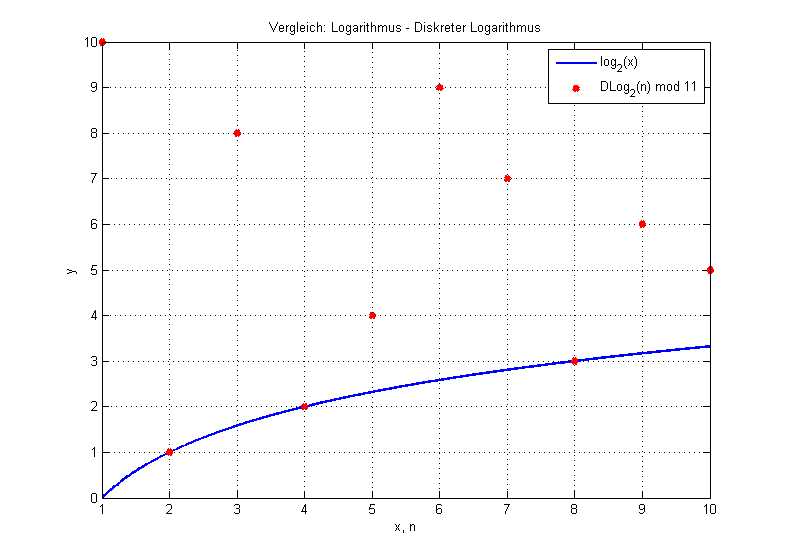
\includegraphics[width=\textwidth]{log_discLog.png}
  \end{center}
\end{frame}

\begin{frame}{Diskretes Logarithmusproblem}
  \begin{itemize}
    \item Sei $p$ eine Primzahl, $g$ ein Erzeuger von $\Z_p^*$ und $y \in
      \Z_p^*$.

      Finde ein $x$ mit $1 \leq x \leq p-1$, so dass $g^x \equiv y \mod
      p$ gilt.
  \end{itemize}
\end{frame}

\section{Praktische Anwendung}
\label{sec:praktische_anwendung}

\subsection{Komplexität}
\label{sub:komplexitat}

\begin{frame}{\insertsubsectionhead}
  Diskreter Logarithmus: $DL(y, g, p) = x$ für $g^x \equiv y \mod p$
  \begin{itemize}
    \item kein direktes Verfahren: Brute Force über $\{1, \ldots, x\}\in
      \mathcal O(x)$
    \item Länge von $x$ in bit: $n \Rightarrow \mathcal{O}(2^n)$
  \end{itemize}

  Angenommen:
  \begin{itemize}
    \item Ein Prozessor mit 10 GHz ($= 10^{10}Hz$), kann mit jedem Schritt eine
      modulare Potenz berechnen: $y \equiv \exp(x,g,p) \equiv g^x\mod p$
    \item Anzahl Prozessoren: $k=10^{10} \Rightarrow 10^{20}$ modulare Potenzen
      pro Sekunde $\approx 2^{67} s^{-1}$
    \item Die Zeit zur Berechnung aller modularen Potenzen: $t=\frac{2^n}{2^{67}\cdot
      s^{-1}}=2^{n-67}\cdot s$
  \end{itemize}

  Man kann $x=2^n$ so setzen, dass $t>t_{\text{Alter des Universums}}$:
  \begin{align*}
    t_{\text{Alter des Universums}} & = 14 \cdot 10^9y \\
    & = 14 \cdot 10^9 \cdot 365 \cdot 24 \cdot 60\cdot 60\cdot s\\
    & \approx 2^{59}\cdot s\\
    59 & = n-67 \Rightarrow n = 59+67 \Rightarrow n=126
  \end{align*}
\end{frame}

\subsection{Diffie-Hellman-Merkle-Schlüsselaustausch (DHKE)}
\label{sub:diffie_hellman_merkle_schlusselaustausch}

\begin{frame}{\insertsubsectionhead}
  \begin{center}
    \begin{tabularx}{\textwidth}{Xcl}
      \textbf{Alice} & & \textbf{Bob}\\\midrule
      $\cdot$ wähle: Primzahl $p$\\
      $\cdot$ finde: Erzeuger $g: g^n \mod p \to \{1, \ldots, p-1\}$\\
      $\cdot$ wähle geheimen Schlüssel: $a \in \{1, \ldots, p-1\}$\\
      $\cdot$ berechne öffentlichen Schlüssel: $A \equiv g^a \mod p$\\
      $\cdot$ sende: $(p, g, A)$ an Bob & $\to$
    \end{tabularx}
  \end{center}

  \pause

  \begin{center}
    \begin{tabularx}{\textwidth}{lcX}
      \textbf{Alice} &  & \multicolumn{1}{r}{\textbf{Bob}}\\\midrule
      & & $\cdot$ wähle: geheimen Schlüssel: $b\in \{ 1 ,\ldots , p - 1 \}$\\
      & & $\cdot$ berechne öffentlichen Schlüssel: $B \equiv g^b \mod p$\\
      & & $\cdot$ berechne geheimen gemeinsamen Schlüssel: $K \equiv A^b \mod p$\\
      & $\leftarrow$ & $\cdot$ sende: $B$ an Alice
    \end{tabularx}
  \end{center}

  \pause

  \begin{center}
    \begin{tabularx}{\textwidth}{Xcl}
      \textbf{Alice} &  & \textbf{Bob}\\\midrule
      $\cdot$ berechne geheimen gemeinsamen Schlüssel: $K \equiv B^a \mod p$
    \end{tabularx}
  \end{center}
\end{frame}

\begin{frame}{\insertsubsectionhead}
  \begin{center}
    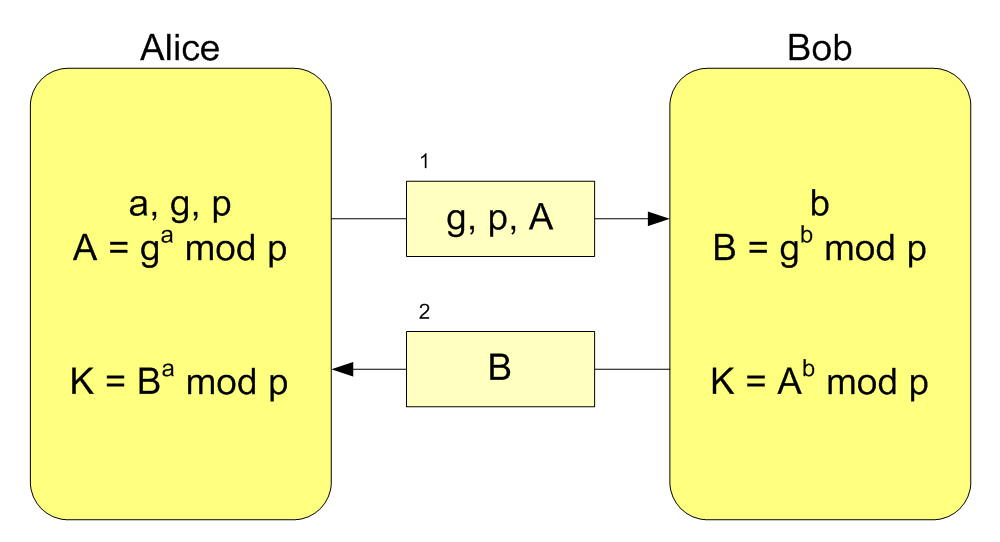
\includegraphics[width=\textwidth]{Diffie-Hellman-Schluesselaustausch2.png}
  \end{center}
  Beweis für Gleichheit der beiden Schlüssel: siehe Tafel
\end{frame}

\subsection{Verschlüsselung mittels DHKE}
\label{sub:verschlusselung_mittels_dhke}

\begin{frame}{\insertsubsectionhead}
  Bob möchte eine Nachricht $m \in \N^n$ an Alice verschicken.

  \pause

  \begin{center}
    \begin{tabularx}{\textwidth}{Xcl}
      \textbf{Alice} & & \textbf{Bob}\\\midrule
      $\cdot$ erzeuge: öffentlichen Schlüssel $(p, g, A)$\\
      $\cdot$ veröffentliche $(p, g, A)$
    \end{tabularx}
  \end{center}

  \pause

  \begin{center}
    \begin{tabularx}{\textwidth}{lcX}
      \textbf{Alice} &  & \multicolumn{1}{r}{\textbf{Bob}}\\\midrule
      & & $\cdot$ wähle: geheimen Schlüssel: $b\in \{ 1 ,\ldots , p - 1 \}$\\
      & & $\cdot$ berechne öffentlichen Schlüssel: $B \equiv g^b \mod p$\\
      & & $\cdot$ verschlüssele: $c_i \equiv A^b \cdot m_i \mod p$\\
      & $\leftarrow$ & $\cdot$ sende: $(B, c)$ an Alice
    \end{tabularx}
  \end{center}

  \pause

  \begin{center}
    \begin{tabularx}{\textwidth}{Xcl}
      \textbf{Alice} &  & \textbf{Bob}\\\midrule
      $\cdot$ entschlüssele: $m_i \equiv B^{-a} \cdot c_i \mod p$\\
      $m_i \equiv B^{(p-1)-a} \cdot c_i \mod p$
    \end{tabularx}
  \end{center}
\end{frame}

\end{document}
